\documentclass[a4paper]{report}
\usepackage{tikz}
\usetikzlibrary{shapes, arrows, positioning}
%\tikzstyle{circle}=[circle, draw, ultra thick, fill=blue!20]

\begin{document}
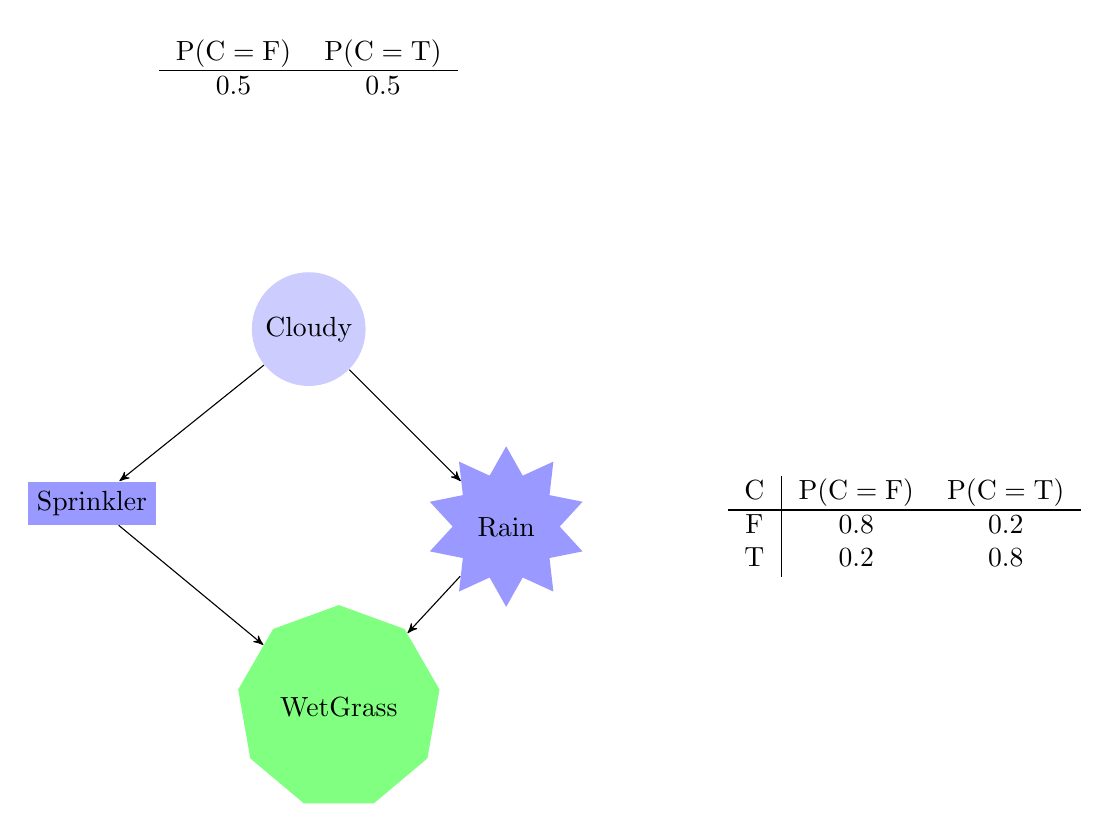
\begin{tikzpicture}[scale=2, node distance=2cm, >=stealth']
\node [circle, fill=blue!20] (cloudy) {Cloudy};
\node [rectangle, fill=blue!40, below left = of cloudy] (sprinkler) {Sprinkler};
\node [star,star points=10, fill=blue!40, below right = of cloudy] (rain) {Rain};
\node [regular polygon,regular polygon sides=9, fill=green!50, below right = of sprinkler] (wetgrass) {WetGrass};

\draw [->] (cloudy) -- (sprinkler);
\draw [->] (cloudy) -- (rain);
\draw [->] (rain) -- (wetgrass);
\draw [->] (sprinkler) -- (wetgrass);

\node [above = of cloudy] {
    \begin{tabular}{cc}
    $\mathrm{P(C=F)}$ & $\mathrm{P(C=T)}$\\
    \hline
    0.5 & 0.5\\
    \end{tabular}
    };

\node [right = of rain, anchor=west] {
    \begin{tabular}{c|cc}
    C & $\mathrm{P(C=F)}$ & $\mathrm{P(C=T)}$\\
    \hline
    F & 0.8 & 0.2\\
    T & 0.2 & 0.8\\
    \end{tabular}
    };  

\end{tikzpicture}
\end{document}
